\section{Evaluation Methodology}
\label{sec:evaluation-methodology}

	% CAP Benchmark justify
	To deliver a comprehensive assessment of \lwmpi, we relied on a
	subset of the CAP Bench suite~\cite{Souza2017}.
	Applications in CAP Bench are developed in the C language, and feature
	different parallel patterns, task types, communication intensity, and
	task loads. The applications employed in our analysis are:
	%
	\begin{description}
		\item[Friendly Numbers (FN)] is an application that finds all
			subsets of numbers in a range $[n,m]$ that share the same
			\textit{abundance}. The abundance of $n$ is the ratio
			between the sum of divisors of $n$ by $n$ itself. FN
			implements the \textit{MapReduce} parallel pattern and has
			tasks with regular loads. The problem is predominantly
			CPU-bound.

		\item[Gaussian Filter (GF)] is a filter that reduces the noise
			of an image by applying a matrix convolution operation with
			a special two-dimensional Gaussian mask to the image pixels.
			GF performs the \textit{Stencil} parallel pattern to
			equal-sized parts of the image, thus being CPU-intensive and
			having a medium communication intensity.

		\item[K-Means (KM)] is a clustering technique employed in
			data analysis. KM gets a set of $n$ points in real
			$d$-dimensional space and randomly split them into $k$
			partitions. Then, it applies the \textit{Map} parallel
			pattern to distribute points and replicate data centroids
			between the \cclusters. The irregular workload is both CPU-
			and memory-bound. Since each iteration must update data
			centroids, this kernel operates with high communication
			intensity.
	\end{description}

	We implemented these applications with \mpi\footnote{Publicly
	available at: \url{https://github.com/nanvix/benchmarks}.} and
	contrasted them with the original implementation of the benchmark for
	\mppa. Noteworthy, \textit{a direct performance comparison between these two
	solutions is unfair}, since the original implementation relies on
	a vendor-specific runtime system, narrowed for
	\mppa, and does not provide any means of software portability across
	architectures.
	%
	% Kernels parameters
	Overall, we carried out strong scaling experiments, where we varied
	the number of workers from 1 to 15, plus a \textit{leader} process that
	coordinates the execution, and we fixed the problem sizes
	of applications as follows:
	%
	\begin{enumerate*}[label=(\roman*)]
		\item numbers ranging from $1000001$ to $1000129$ for FN;
		\item $512\times512$ image and $7\times$ mask for GF; and
		\item 30720 points and 64 centroids for KM.
	\end{enumerate*}
	%
	We ran 30 trials of each configuration to ensure minimum variance, and
	the maximum coefficient of variance observed was below 1\%.

	%
	% MPPA-256
	\subsection{Experimental Platform}

	The \mppa is an example of an industry-successful lightweight
	manycore, and Figure \ref{figure:lightweight-manycore} presents its
	architectural blueprint.
	%
	Overall, it integrates 288 cores disposed into 20
	clusters. Each cluster is composed of heterogeneous
	hardware capabilities to perform different roles. For instance,
	\ioclusters have four \rmans, four \noc interfaces, and 4~MB local
	\sram to exchange data with external resources and internal clusters.
	Differently, \cclusters have one \rman, 16 \pes, one \noc interface,
	and only 2~MB local \sram to run user workloads. Cores within the
	cluster share and have uniform access to hardware resources.

	% Network-On-Chip
	Communication between clusters is exclusively achieved by explicitly
	exchanging hardware-level messages through two \nocs. Specifically,
	the \cnoc enables synchronization and small control messages handover,
	whereas the \dnoc supports arbitrary-sized data exchanges.
	\ioclusters have direct access to the attached \dram or a device,
	while \cclusters must tile their data into messages and send them
	through the \noc using an \iocluster as an intermediary to access
	these resources. \mppa also features
	a built-in \dma engine in its \noc interfaces to enable asynchronous
	communications and higher bandwidth for dense data transfers.

	\begin{figure}[t]
		\centering
		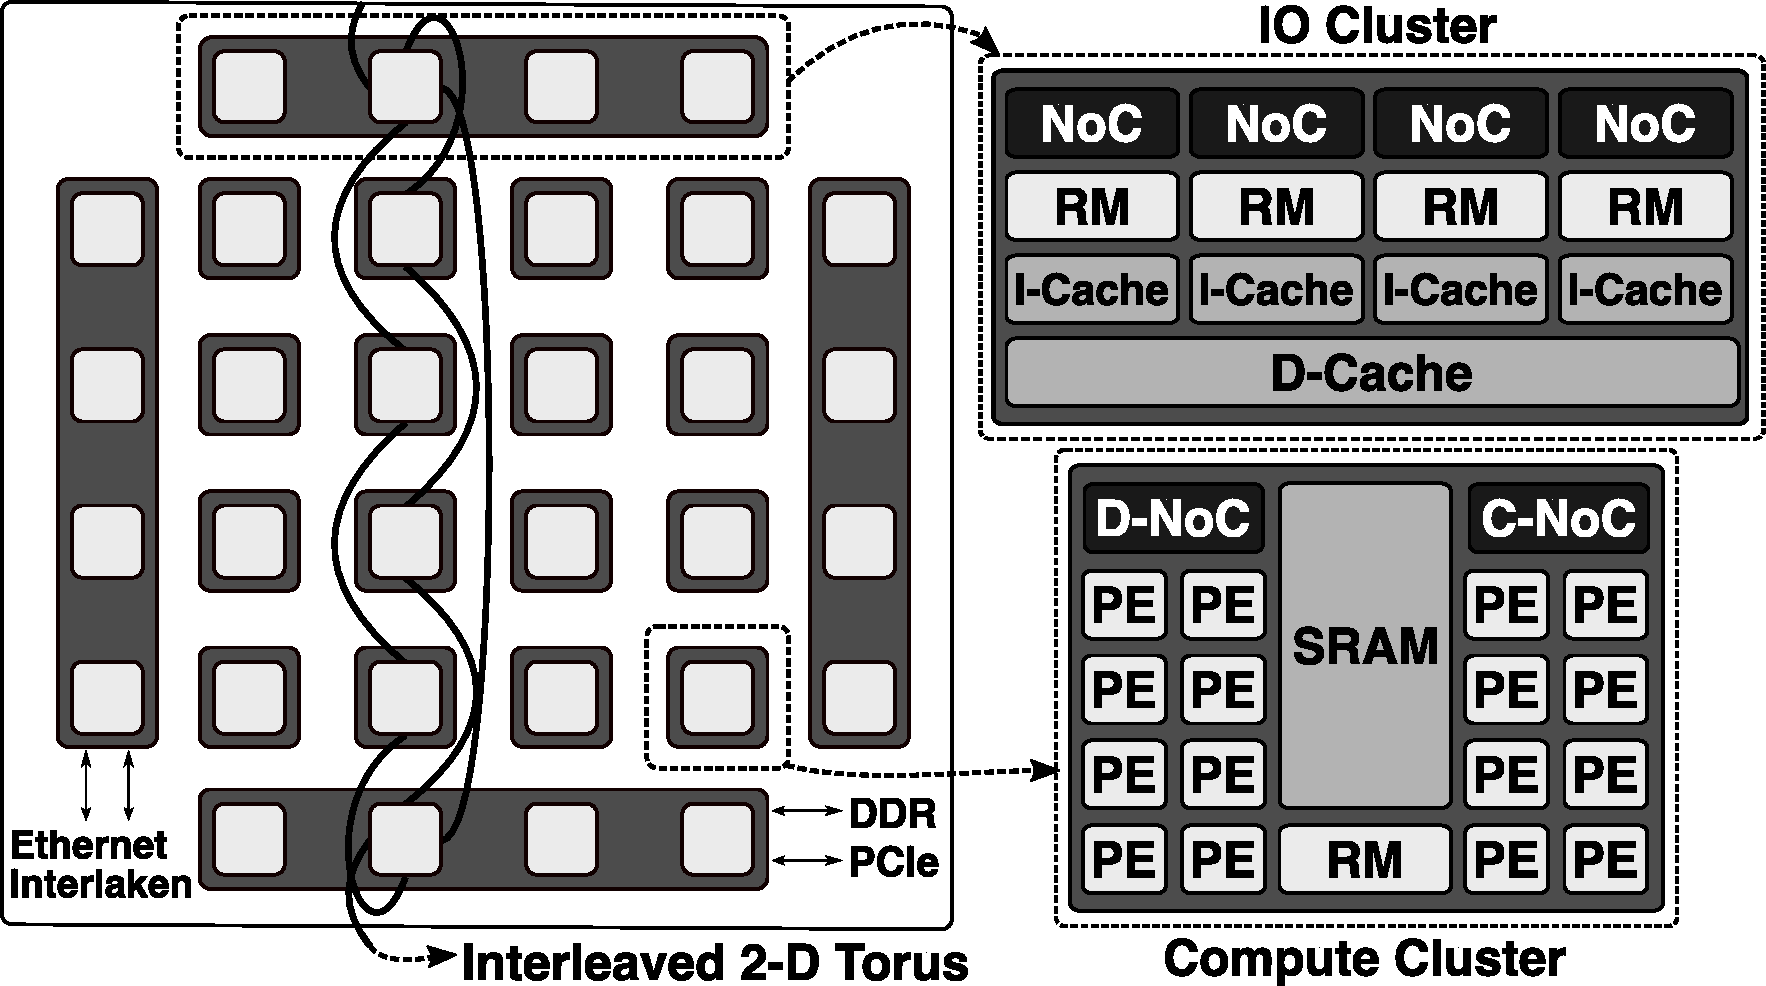
\includegraphics[width=.8\linewidth]{mppa256}
		\caption{\mppa architectural overview.}
		\label{figure:lightweight-manycore}
		\vspace{-15pt}
	\end{figure}
